\section{Date: 2026-11-03}
\noindent \textbf{Series ID: AITINO} 

\noindent This series is titled Manufacturers' New Orders: Information Technology Industries and has a frequency of Monthly. The units are Millions of Dollars and the seasonal adjustment is Seasonally Adjusted.The observation start date is 1992-02-01 and the observation end date is 2026-09-01.The popularity of this series is 14. \\ 

\noindent \textbf{Series ID: MOROE} 

\noindent This series is titled Return on Average Equity for Banks in Missouri (DISCONTINUED) and has a frequency of Quarterly, End of Period. The units are Percent and the seasonal adjustment is Not Seasonally Adjusted.The observation start date is 1984-01-01 and the observation end date is 2020-07-01.The popularity of this series is 1. \\ 

\subsection{Raw Regression}
\noindent Regresses the two series against each other directly. A significant result here can come just as easily from both series sharing a long-run trend as from any real relationship.

\begin{center}
\begin{tabular}{lclc}
\toprule
\textbf{Dep. Variable:}      & value\_fred\_MOROE & \textbf{  R-squared:         } &     0.135   \\
\textbf{Model:}              &        OLS         & \textbf{  Adj. R-squared:    } &     0.128   \\
\textbf{Method:}             &   Least Squares    & \textbf{  F-statistic:       } &     17.51   \\
\textbf{Date:}               &  Tue, 03 Nov 2026  & \textbf{  Prob (F-statistic):} &  5.69e-05   \\
\textbf{Time:}               &      18:56:19      & \textbf{  Log-Likelihood:    } &   -307.15   \\
\textbf{No. Observations:}   &          114       & \textbf{  AIC:               } &     618.3   \\
\textbf{Df Residuals:}       &          112       & \textbf{  BIC:               } &     623.8   \\
\textbf{Df Model:}           &            1       & \textbf{                     } &             \\
\textbf{Covariance Type:}    &     nonrobust      & \textbf{                     } &             \\
\bottomrule
\end{tabular}
\begin{tabular}{lcccccc}
                             & \textbf{coef} & \textbf{std err} & \textbf{t} & \textbf{P$> |$t$|$} & \textbf{[0.025} & \textbf{0.975]}  \\
\midrule
\textbf{const}               &       1.9234  &        2.332     &     0.825  &         0.411        &       -2.697    &        6.544     \\
\textbf{value\_fred\_AITINO} &       0.0004  &     9.45e-05     &     4.185  &         0.000        &        0.000    &        0.001     \\
\bottomrule
\end{tabular}
\begin{tabular}{lclc}
\textbf{Omnibus:}       & 41.602 & \textbf{  Durbin-Watson:     } &    0.161  \\
\textbf{Prob(Omnibus):} &  0.000 & \textbf{  Jarque-Bera (JB):  } &   88.948  \\
\textbf{Skew:}          & -1.485 & \textbf{  Prob(JB):          } & 4.84e-20  \\
\textbf{Kurtosis:}      &  6.147 & \textbf{  Cond. No.          } & 1.70e+05  \\
\bottomrule
\end{tabular}
%\caption{OLS Regression Results}
\end{center}

Notes: \newline
 [1] Standard Errors assume that the covariance matrix of the errors is correctly specified. \newline
 [2] The condition number is large, 1.7e+05. This might indicate that there are \newline
 strong multicollinearity or other numerical problems.

\begin{figure}
\centering
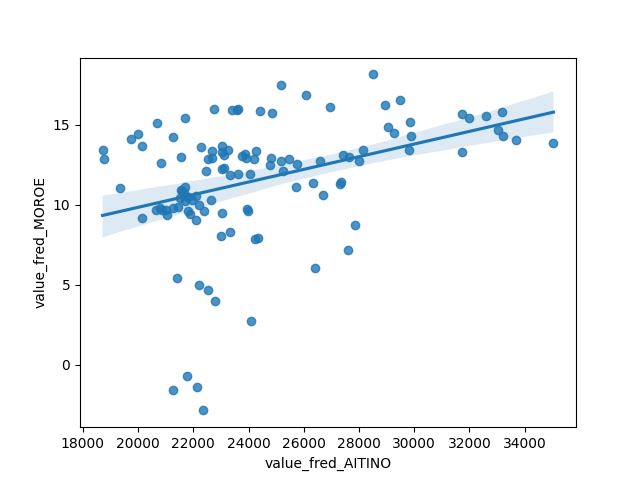
\includegraphics[scale = 0.9]{plots/plot_2026-11-03.png}
\caption{Raw Regression Plot for 2026-11-03}
\end{figure}
\newpage
\subsection{Detrended Regression}
\noindent Regresses the residuals of each series after removing its own linear time trend, so a shared trend can no longer drive the result on its own. A relationship that stays significant here is better evidence of a genuine link between the two series.

\begin{center}
\begin{tabular}{lclc}
\toprule
\textbf{Dep. Variable:}                 & value\_fred\_MOROE\_detrended & \textbf{  R-squared:         } &     0.057   \\
\textbf{Model:}                         &              OLS              & \textbf{  Adj. R-squared:    } &     0.049   \\
\textbf{Method:}                        &         Least Squares         & \textbf{  F-statistic:       } &     6.779   \\
\textbf{Date:}                          &        Tue, 03 Nov 2026       & \textbf{  Prob (F-statistic):} &   0.0105    \\
\textbf{Time:}                          &            18:56:19           & \textbf{  Log-Likelihood:    } &   -295.86   \\
\textbf{No. Observations:}              &                114            & \textbf{  AIC:               } &     595.7   \\
\textbf{Df Residuals:}                  &                112            & \textbf{  BIC:               } &     601.2   \\
\textbf{Df Model:}                      &                  1            & \textbf{                     } &             \\
\textbf{Covariance Type:}               &           nonrobust           & \textbf{                     } &             \\
\bottomrule
\end{tabular}
\begin{tabular}{lcccccc}
                                        & \textbf{coef} & \textbf{std err} & \textbf{t} & \textbf{P$> |$t$|$} & \textbf{[0.025} & \textbf{0.975]}  \\
\midrule
\textbf{const}                          &   -7.674e-13  &        0.306     &  -2.5e-12  &         1.000        &       -0.607    &        0.607     \\
\textbf{value\_fred\_AITINO\_detrended} &       0.0002  &     9.13e-05     &     2.604  &         0.010        &     5.68e-05    &        0.000     \\
\bottomrule
\end{tabular}
\begin{tabular}{lclc}
\textbf{Omnibus:}       & 60.278 & \textbf{  Durbin-Watson:     } &    0.190  \\
\textbf{Prob(Omnibus):} &  0.000 & \textbf{  Jarque-Bera (JB):  } &  192.530  \\
\textbf{Skew:}          & -1.974 & \textbf{  Prob(JB):          } & 1.56e-42  \\
\textbf{Kurtosis:}      &  7.994 & \textbf{  Cond. No.          } & 3.35e+03  \\
\bottomrule
\end{tabular}
%\caption{OLS Regression Results}
\end{center}

Notes: \newline
 [1] Standard Errors assume that the covariance matrix of the errors is correctly specified. \newline
 [2] The condition number is large, 3.35e+03. This might indicate that there are \newline
 strong multicollinearity or other numerical problems.

\begin{figure}
\centering
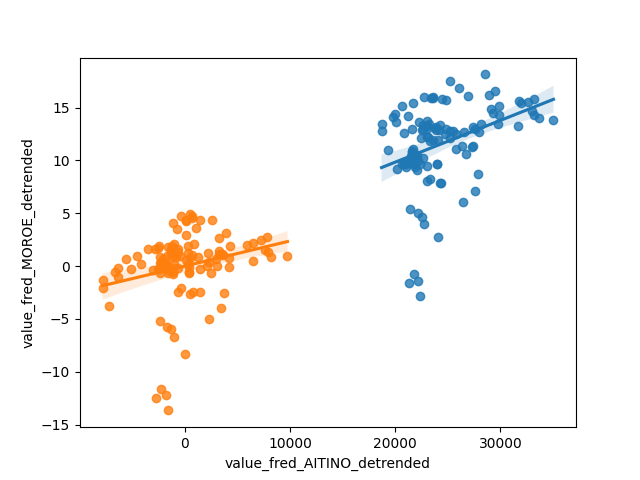
\includegraphics[scale = 0.9]{plots/plot_2026-11-03_detrended.png}
\caption{Detrended Regression Plot for 2026-11-03}
\end{figure}
\newpage
